\documentclass[conference]{IEEEtran}
\usepackage[utf8]{inputenc}
\usepackage{graphicx} % For including figures (like block diagrams)
\usepackage{amsmath}  % For math formulas
\usepackage{listings} % For embedding code snippets
\usepackage{xcolor}   % For colored text in code listings
\usepackage{hyperref} % For clickable links (e.g., in table of contents, citations)
\usepackage{cite}     % For IEEE style citations
\usepackage{tikz}     % Para diagramas
\usetikzlibrary{shapes,arrows,positioning,calc,shapes.geometric}

% IEEEtran specific configurations (optional, can be adjusted)
\IEEEoverridecommandlockouts % To enable \thanks if needed

% Code listing style (example)
\lstdefinestyle{verilogstyle}{
    language=Verilog,
    basicstyle=\ttfamily\footnotesize,
    keywordstyle=\color{blue},
    commentstyle=\color{green!40!black},
    stringstyle=\color{red},
    numbers=left,
    numberstyle=\tiny\color{gray},
    breaklines=true,
    breakatwhitespace=true,
    tabsize=2,
    captionpos=b, % caption below the listing
    frame=single, % adds a frame around the code
    rulecolor=\color{black!30!white}, % frame color
    backgroundcolor=\color{black!5!white} % background color
}
\lstset{style=verilogstyle}

\title{Diseño e Implementación de un Procesador RISC-V Uniciclo}
% \author{Your Name/Group Name Here} % We can add this later
\date{\today}

\begin{document}

\maketitle
\begin{abstract}
This document details the design and implementation of a single-cycle RISC-V processor with a modular architecture. The new design separates the datapath, control unit, and ALU control into distinct modules, improving clarity, scalability, and maintainability. The document covers the architectural overview, the functionality of individual modules such as the Program Counter, Instruction Memory, Register File, ALU, Data Memory, Sign Extension unit, Datapath, Control Unit, and ALU Control. The new control logic is fully combinational, generating all control signals explicitly for each instruction type. The integration of jump instructions and modular control is described in detail.
\end{abstract}

\begin{IEEEkeywords}
RISC-V, Unicycle Processor, Computer Architecture, SystemVerilog, HDL.
\end{IEEEkeywords}

\section{Introducción}
\label{sec:introduction}
Este informe presenta el diseño e implementación de un procesador RISC-V de 32 bits con arquitectura uniciclo. El procesador está descrito en SystemVerilog e incluye los módulos esenciales necesarios para la obtención, decodificación y ejecucion de un subconjunto de la arquitectura de conjunto de instrucciones (ISA) RISC-V.
El objetivo principal de este proyecto es demostrar el funcionamiento de un camino de datos y unidad de control uniciclo. Este documento detalla el marco teórico, la arquitectura general del sistema, el diseño detallado de cada módulo hardware y el conjunto de instrucciones soportado.

\section{Marco Teórico}
\label{sec:theoretical_framework}
\subsection{Arquitectura RISC-V}
La ISA RISC-V es una arquitectura de conjunto de instrucciones de código abierto basada en los principios establecidos de computadoras con conjunto reducido de instrucciones (RISC). Su diseño modular permite una ISA base entera con extensiones opcionales para diversas necesidades computacionales. Este proyecto implementa un subconjunto del conjunto base entero RV32I.

\subsection{Procesador Uniciclo}
Un procesador uniciclo ejecuta cada instruccion en un solo ciclo de reloj. Esta filosofía de diseño simplifica la unidad de control, pero puede resultar en un ciclo de reloj más largo, ya que debe acomodar el camino crítico de la instruccion más compleja. Los componentes del camino de datos operan en paralelo dentro de ese único ciclo.

\subsection{Referencias clave}
Los principios de diseño y conceptos específicos de RISC-V discutidos en este documento están fuertemente influenciados por la literatura clásica de arquitectura de computadoras, en particular la obra de Patterson y Hennessy \cite{PattersonHennessy2021RISCV}.

\section{Arquitectura del Sistema}
\label{sec:system_architecture}
\subsection{Camino de Datos General y Modulo Datapath}
El camino de datos esta ahora abstraído en el modulo \texttt{datapath.sv}, que integra los modulos esenciales: Program Counter (PC), Memoria de Instrucciones, Banco de Registros, Unidad de Extension de Signo, ALU y Memoria de Datos. El datapath recibe todas las senales de control desde la unidad de control externa y ejecuta la instruccion correspondiente en un solo ciclo.

La logica de seleccion de operandos para la ALU y la actualizacion del PC ahora depende de senales externas como \texttt{jal\_active} y \texttt{jalr\_active}, permitiendo un control claro y modular de los saltos y flujos de ejecucion.

\textbf{Seleccion de operandos para saltos:}
\begin{lstlisting}[language=Verilog, caption={Seleccion de operandos en datapath.sv}]
always_comb begin
    if (jal_active && !jalr_active) begin
        alu_input_a = pc_current_val;
        alu_input_b = sign_extended_imm;
    end else if (!jal_active && jalr_active) begin
        alu_input_a = reg_data_1;
        alu_input_b = sign_extended_imm;
    end else begin
        alu_input_a = reg_data_1;
        alu_input_b = alu_src_b ? sign_extended_imm : reg_data_2;
    end
end
\end{lstlisting}

El resultado de la ALU se utiliza para actualizar el PC en instrucciones de salto, asegurando la correcta ejecucion de JAL y JALR.

\begin{figure*}[!t]
    \centering
    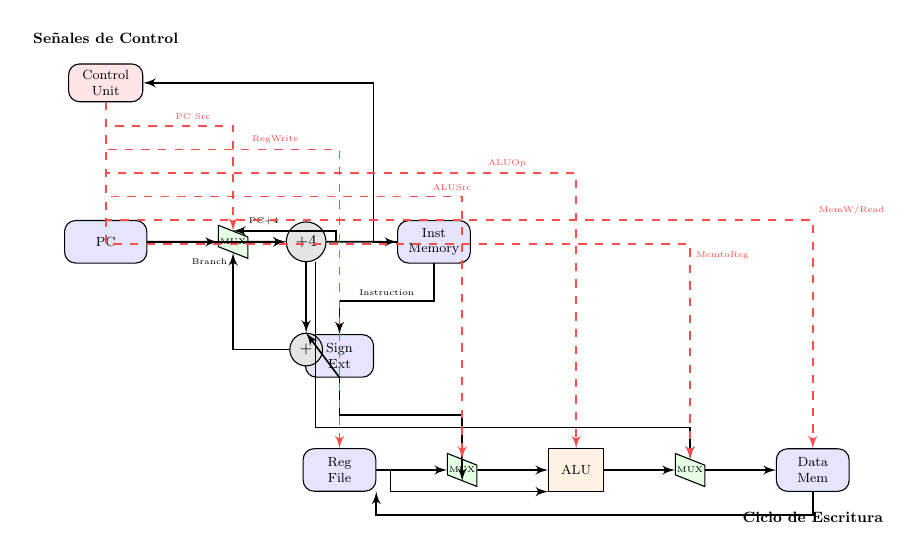
\begin{tikzpicture}[
        node distance=1cm and 1.5cm,
        block/.style={
            rectangle, 
            draw, 
            fill=blue!10, 
            text width=1.6cm, 
            text centered, 
            rounded corners, 
            minimum height=0.9cm,
            font=\footnotesize,
            inner sep=2pt
        },
        mux/.style={
            trapezium, 
            trapezium left angle=70, 
            trapezium right angle=-70, 
            draw, 
            fill=green!10, 
            minimum width=0.7cm, 
            minimum height=0.6cm, 
            inner sep=1pt, 
            shape border rotate=90, 
            trapezium stretches=true,
            font=\tiny
        },
        control/.style={
            rectangle, 
            draw, 
            fill=red!10, 
            text width=1.5cm, 
            text centered, 
            rounded corners, 
            minimum height=0.8cm,
            font=\footnotesize,
            inner sep=1pt
        },
        alu/.style={
            rectangle, 
            draw, 
            fill=orange!10, 
            text width=1.1cm, 
            text centered, 
            minimum height=0.9cm,
            font=\footnotesize,
            inner sep=1pt
        },
        line/.style={
            draw, 
            -latex',
            >=stealth,
            line width=0.6pt
        },
        dashedline/.style={
            draw, 
            -latex', 
            dashed, 
            red!70,
            >=stealth,
            line width=0.6pt
        },
        datalabel/.style={
            font=\tiny, 
            near start, 
            sloped, 
            above,
            text=black
        },
        scale=0.6,
        transform shape,
        every node/.style={transform shape}
    ]
    
    % === Nodos principales - Primera Fila (Arriba) ===
    % Unidad de control
    \node [control] (control) {Control\\Unit};
    
    % === Segunda Fila ===
    % PC
    \node [block, below=2.5cm of control] (pc) {PC};
    
    % MUX del PC
    \node [mux, right=1.5cm of pc] (mux_pc) {MUX};
    
    % Sumador +4
    \node [draw, circle, fill=gray!20, right=0.8cm of mux_pc, minimum size=0.5cm] (add4) {+4};
    
    % Memoria de instrucciones
    \node [block, right=1.5cm of add4, text width=1.4cm] (instmem) {Inst\\Memory};
    
    % === Tercera Fila ===
    % Extensor de signo
    \node [block, below=1.5cm of instmem, xshift=-2cm, text width=1.3cm] (signext) {Sign\\Ext};
    
    % Sumador de branch
    \node [draw, circle, fill=gray!20, below=1.5cm of add4, minimum size=0.5cm] (add_branch) {+};
    
    % === Cuarta Fila ===
    % Banco de registros
    \node [block, below=1.5cm of signext, text width=1.4cm] (regfile) {Reg\\File};
    
    % MUX ALU B
    \node [mux, right=1.5cm of regfile] (mux_alu_b) {MUX};
    
    % ALU
    \node [alu, right=1.5cm of mux_alu_b] (alu) {ALU};
    
    % MUX Write Back
    \node [mux, right=1.5cm of alu] (mux_wb) {MUX};
    
    % Memoria de datos
    \node [block, right=1.5cm of mux_wb, text width=1.4cm] (datamem) {Data\\Mem};
    
    % === Conexiones principales ===
    % PC -> MUX PC
    \draw [line] (pc.east) -- (mux_pc.west);
    
    % MUX PC -> InstMem
    \draw [line] (mux_pc.east) -- (add4.west);
    \draw [line] (add4.east) -- (instmem.west);
    
    % PC -> +4 (conexión directa al sumador +4)
    \draw [line] (pc.east) -- ++(0.5,0) |- (add4.west);
    
    % +4 -> MUX PC (PC+4)
    \draw [line] (add4.east) ++(0.2,0) |- (mux_pc.north) node[above left, font=\tiny, pos=0.75] {PC+4};
    
    % === Tercera fila de conexiones ===
    % InstMem -> Banco de registros
    \draw [line] (instmem.south) -- ++(0,-0.8) -| (signext.north) 
        node[pos=0.25, above, font=\tiny] {Instruction};
    
    % InstMem -> Extensor de signo (ya conectado arriba)
    
    % InstMem -> Unidad de control
    \draw [line] (instmem.west) -- ++(-0.5,0) |- (control.east);
    
    % Extensor -> Sumador branch
    \draw [line] (signext.south) -- (add_branch.north);
    
    % +4 -> Sumador branch (conexión desde add4)
    \draw [line] (add4.south) -- ++(0,-0.5) -| (add_branch.north);
    
    % Sumador branch -> MUX PC (Branch Target)
    \draw [line] (add_branch.west) -| (mux_pc.south) node[below left, font=\tiny] {Branch};
    
    % === Cuarta fila de conexiones ===
    % Banco de registros -> MUX ALU B
    \draw [line] (regfile.east) -- ++(0.3,0) |- (mux_alu_b.west);
    
    % Banco de registros -> ALU
    \draw [line] (regfile.east) ++(0.3,0) |- (alu.south west);
    
    % Extensor de signo -> MUX ALU B
    \draw [line] (signext.south) -- ++(0,-0.8) -| (mux_alu_b.south);
    
    % MUX ALU B -> ALU
    \draw [line] (mux_alu_b.east) -- (alu.west);
    
    % ALU -> MUX WB
    \draw [line] (alu.east) -- (mux_wb.west);
    
    % MUX WB -> Memoria de datos
    \draw [line] (mux_wb.east) -- (datamem.west);
    
    % Memoria de datos -> Banco de registros (Write Back)
    \draw [line] (datamem.south) -- ++(0,-0.5) -| (regfile.south east);
    
    % +4 -> MUX WB (para jal)
    \draw [line] (add4.south) ++(0.2,0) -- ++(0,-3.5) -| (mux_wb.north);
    
    % === Señales de control ===
    % Unidad de control -> MUX PC
    \draw [dashedline] (control.south) -- ++(0,-0.5) -| (mux_pc.north) 
        node[above right, font=\tiny, pos=0.25] {PC Src};
    
    % Unidad de control -> Banco de registros
    \draw [dashedline] (control.south) -- ++(0,-1) -| (regfile.north) 
        node[above right, font=\tiny, pos=0.3] {RegWrite};
    
    % Unidad de control -> ALU
    \draw [dashedline] (control.south) -- ++(0,-1.5) -| (alu.north) 
        node[above right, font=\tiny, pos=0.4] {ALUOp};
    
    % Unidad de control -> MUX ALU B
    \draw [dashedline] (control.south) -- ++(0,-2) -| (mux_alu_b.north) 
        node[above right, font=\tiny, pos=0.45] {ALUSrc};
    
    % Unidad de control -> Memoria de datos
    \draw [dashedline] (control.south) -- ++(0,-2.5) -| (datamem.north) 
        node[above right, font=\tiny, pos=0.5] {MemW/Read};
    
    % Unidad de control -> MUX WB
    \draw [dashedline] (control.south) -- ++(0,-3) -| (mux_wb.north) 
        node[above right, font=\tiny, pos=0.55] {MemtoReg};
    
    % === Etiquetas ===
    \node[above=0.3cm of control, font=\small\bfseries] {Señales de Control};
    \node[below=0.3cm of datamem, font=\small\bfseries] {Ciclo de Escritura};
    \end{tikzpicture}
    \caption{Diagrama de bloques del procesador RISC-V uniciclo. Se muestran los módulos principales: PC, Memoria de Instrucciones, Banco de Registros, ALU, Memoria de Datos, Extensor de Signo y la Unidad de Control. Las líneas continuas representan el flujo de datos, mientras que las líneas punteadas en rojo representan las señales de control generadas por la Unidad de Control.}
    \label{fig:diagrama_bloques}
\end{figure*}

\subsection{Unidad de Control (control\_unit.sv)}
La unidad de control es ahora un modulo independiente y completamente combinacional. Recibe los campos opcode, funct3 y funct7 de la instruccion y genera de manera explicita todas las senales de control necesarias para el datapath. Entre las senales generadas se encuentran la seleccion de operacion de la ALU, habilitacion de escritura en registros, control de acceso a memoria, seleccion de fuente de datos para escritura en registros, y senales especificas para instrucciones de salto (\texttt{jal\_active}, \texttt{jalr\_active}).

Cada instruccion tiene asignaciones explicitas para todas las senales de control, evitando valores indeterminados. La unidad de control centraliza la decodificacion y facilita la extension o modificacion del conjunto de instrucciones soportadas.

\textbf{Ejemplo de generacion de senales para JAL y JALR:}
Ejemplo de señales de control para JAL/JALR omitido por problemas de formato. Ver código fuente.

La unidad de control se conecta al datapath a través de todas las senales de control, incluyendo las de salto.

\section{Descripción de Módulos}
\label{sec:module_descriptions}

\subsection{Contador de Programa (PC.sv)}
El módulo Program Counter (PC) es responsable de mantener la direccion de la instruccion que está siendo obtenida.
\subsubsection{Entradas}
\begin{itemize}
    \item \texttt{clk}: Señal de reloj.
    \item \texttt{reset}: Señal de reset asíncrono.
    \item \texttt{branch}: Señal de control para instrucciones de salto.
    \item \texttt{branch\_offset}: Desplazamiento con signo de 32 bits para instrucciones de salto.
    \item \texttt{finish\_flag}: Bandera que indica finalización del programa.
\end{itemize}
\subsubsection{Salidas}
\begin{itemize}
    \item \texttt{pc\_reg}: Valor actual del contador de programa (32 bits).
\end{itemize}
\subsubsection{Funcionamiento}
Al hacer reset, el PC se inicializa a \texttt{32'hFFFFFFFC}. En cada ciclo de reloj, si no hay salto y el programa no ha terminado, el PC se incrementa en 4. Si se toma un salto (\texttt{branch} en alto), \texttt{pc\_reg} se actualiza a la suma del PC actual y \texttt{branch\_offset}.

\subsection{Memoria de Instrucciones (Instmemory.sv)}
Este módulo almacena las instrucciones del programa.
\subsubsection{Entradas}
\begin{itemize}
    \item \texttt{addr}: Dirección de 32 bits proveniente del PC.
\end{itemize}
\subsubsection{Salidas}
\begin{itemize}
    \item \texttt{instruct}: Instrucción de 32 bits obtenida de la direccion indicada.
    \item \texttt{last\_instr\_flag}: Bandera que se activa si la instruccion obtenida es \texttt{32'hFFFFFFFF}.
\end{itemize}
\subsubsection{Funcionamiento}
Inicializa su contenido desde el archivo \texttt{Test1.hex}. Proporciona la instruccion ubicada en la direccion de byte especificada por \texttt{addr}. La memoria se implementa como un arreglo de bytes y cuatro bytes se concatenan para formar la instruccion de 32 bits. La bandera \texttt{last\_instr\_flag} es utilizada por el módulo de control principal para detectar el fin del programa.

\subsection{Banco de Registros (registerfile.sv)}
El banco de registros contiene los 32 registros de propósito general del procesador.
\subsubsection{Entradas}
\begin{itemize}
    \item \texttt{Read1}, \texttt{Read2}: Direcciones de 5 bits para los registros a leer.
    \item \texttt{RD}: Dirección de 5 bits para el registro a escribir.
    \item \texttt{WriteData}: Dato de 32 bits a escribir en el banco de registros.
    \item \texttt{RegWrite}: Señal de control que habilita la escritura.
    \item \texttt{clock}: Señal de reloj (aunque la escritura parece ser combinacional con \texttt{WriteData} en el código, típicamente es sincronizada).
    \item \texttt{finish\_flag}: Bandera de finalización del programa.
\end{itemize}
\subsubsection{Salidas}
\begin{itemize}
    \item \texttt{Data1}, \texttt{Data2}: Datos de 32 bits leídos de los registros especificados por \texttt{Read1} y \texttt{Read2}.
\end{itemize}
\subsubsection{Funcionamiento}
Permite dos lecturas simultáneas y una escritura. El registro \texttt{x0} está cableado a cero (inicializado en 0 y típicamente no se escribe por convención RISC-V). La escritura ocurre si \texttt{RegWrite} está activa y el programa no ha terminado (verificado con \texttt{finish\_flag}). Algunos registros se inicializan con valores específicos para pruebas.

\subsection{Unidad de Extensión de Signo (signext.sv)}
Este módulo extiende los valores inmediatos de las instrucciones a 32 bits.
\subsubsection{Entradas}
\begin{itemize}
    \item \texttt{instruct}: Instrucción de 32 bits que contiene el campo inmediato.
\end{itemize}
\subsubsection{Salidas}
\begin{itemize}
    \item \texttt{out}: Valor inmediato extendido a 32 bits con signo.
\end{itemize}
\subsubsection{Funcionamiento}
Determina el tipo de inmediato según el opcode (bits 6:0) de la instruccion y realiza la extensión de signo correspondiente para inmediatos tipo I, S y B. Para instrucciones de carga (opcode \texttt{7'b0000011}), también realiza extensión tipo I.

\subsection{Unidad de Control de la ALU (alu\_control.sv)}
El módulo \texttt{alu\_control.sv} traduce el opcode, funct3 y funct7 de la instruccion en una senal de control de 4 bits para la ALU. Esto permite que la ALU soporte múltiples operaciones aritméticas y lógicas, así como el calculo de direcciones para saltos. La lógica de decodificación de la operacion de la ALU está completamente separada de la unidad de control principal, facilitando la extensión del conjunto de operaciones soportadas.

\textbf{Ejemplo de decodificación:}
\textit{Fragmento de código omitido por problemas de formato. Consulte el archivo fuente para más detalles.}

\subsection{Unidad Aritmético-Lógica (RISCVALU.sv)}
La ALU realiza operaciones aritméticas y lógicas.
\subsubsection{Entradas}
\begin{itemize}
    \item \texttt{ALUctl}: Señal de control de 4 bits que especifica la operacion.
    \item \texttt{A}, \texttt{B}: Operandos de 32 bits.
    \item \texttt{reset\_zero\_flag}: Señal para reiniciar la bandera interna zero.
\end{itemize}
\subsubsection{Salidas}
\begin{itemize}
    \item \texttt{ALUout}: Resultado de la operacion (32 bits).
    \item \texttt{zero}: Bandera que se activa si el resultado de una resta (A-B) es cero.
\end{itemize}
\subsubsection{Funcionamiento}
Las operaciones soportadas incluyen AND, OR, ADD, SUB y SLT (Set Less Than). La bandera \texttt{zero} se actualiza específicamente tras una resta si el resultado es cero y puede ser reiniciada mediante \texttt{reset\_zero\_flag}.

\subsection{Memoria de Datos (datamem.sv)}
La memoria de datos se utiliza para operaciones de carga y almacenamiento.
\subsubsection{Entradas}
\begin{itemize}
    \item \texttt{clk}: Señal de reloj.
    \item \texttt{address}: Dirección de 32 bits para acceso a memoria.
    \item \texttt{write\_data}: Dato de 32 bits para operaciones de almacenamiento.
    \item \texttt{write\_enable}: Señal de control para habilitar escritura.
    \item \texttt{read\_enable}: Señal de control para habilitar lectura.
\end{itemize}
\subsubsection{Salidas}
\begin{itemize}
    \item \texttt{read\_data}: Dato de 32 bits leído de memoria para operaciones de carga.
\end{itemize}
\subsubsection{Funcionamiento}
Modela una memoria de 256 palabras de 32 bits. Inicializa su contenido desde \texttt{ProyectoCorto\_data.hex}. Las operaciones de escritura se realizan en el flanco positivo del reloj si \texttt{write\_enable} está activa. Las operaciones de lectura también son síncronas, proporcionando \texttt{read\_data} según la direccion si \texttt{read\_enable} está activa.

\subsection{Módulo Principal (RISCVunicycle.sv)}
Este módulo de nivel superior integra todos los componentes y conecta explícitamente la unidad de control, el datapath y el \texttt{alu\_control}. La lógica de control ya no está embebida ni secuencial, sino completamente modular y conectada por señales explícitas. El top module se encarga de enrutar las señales de control y datos entre los módulos principales.

\begin{figure}[h!]
    \centering
    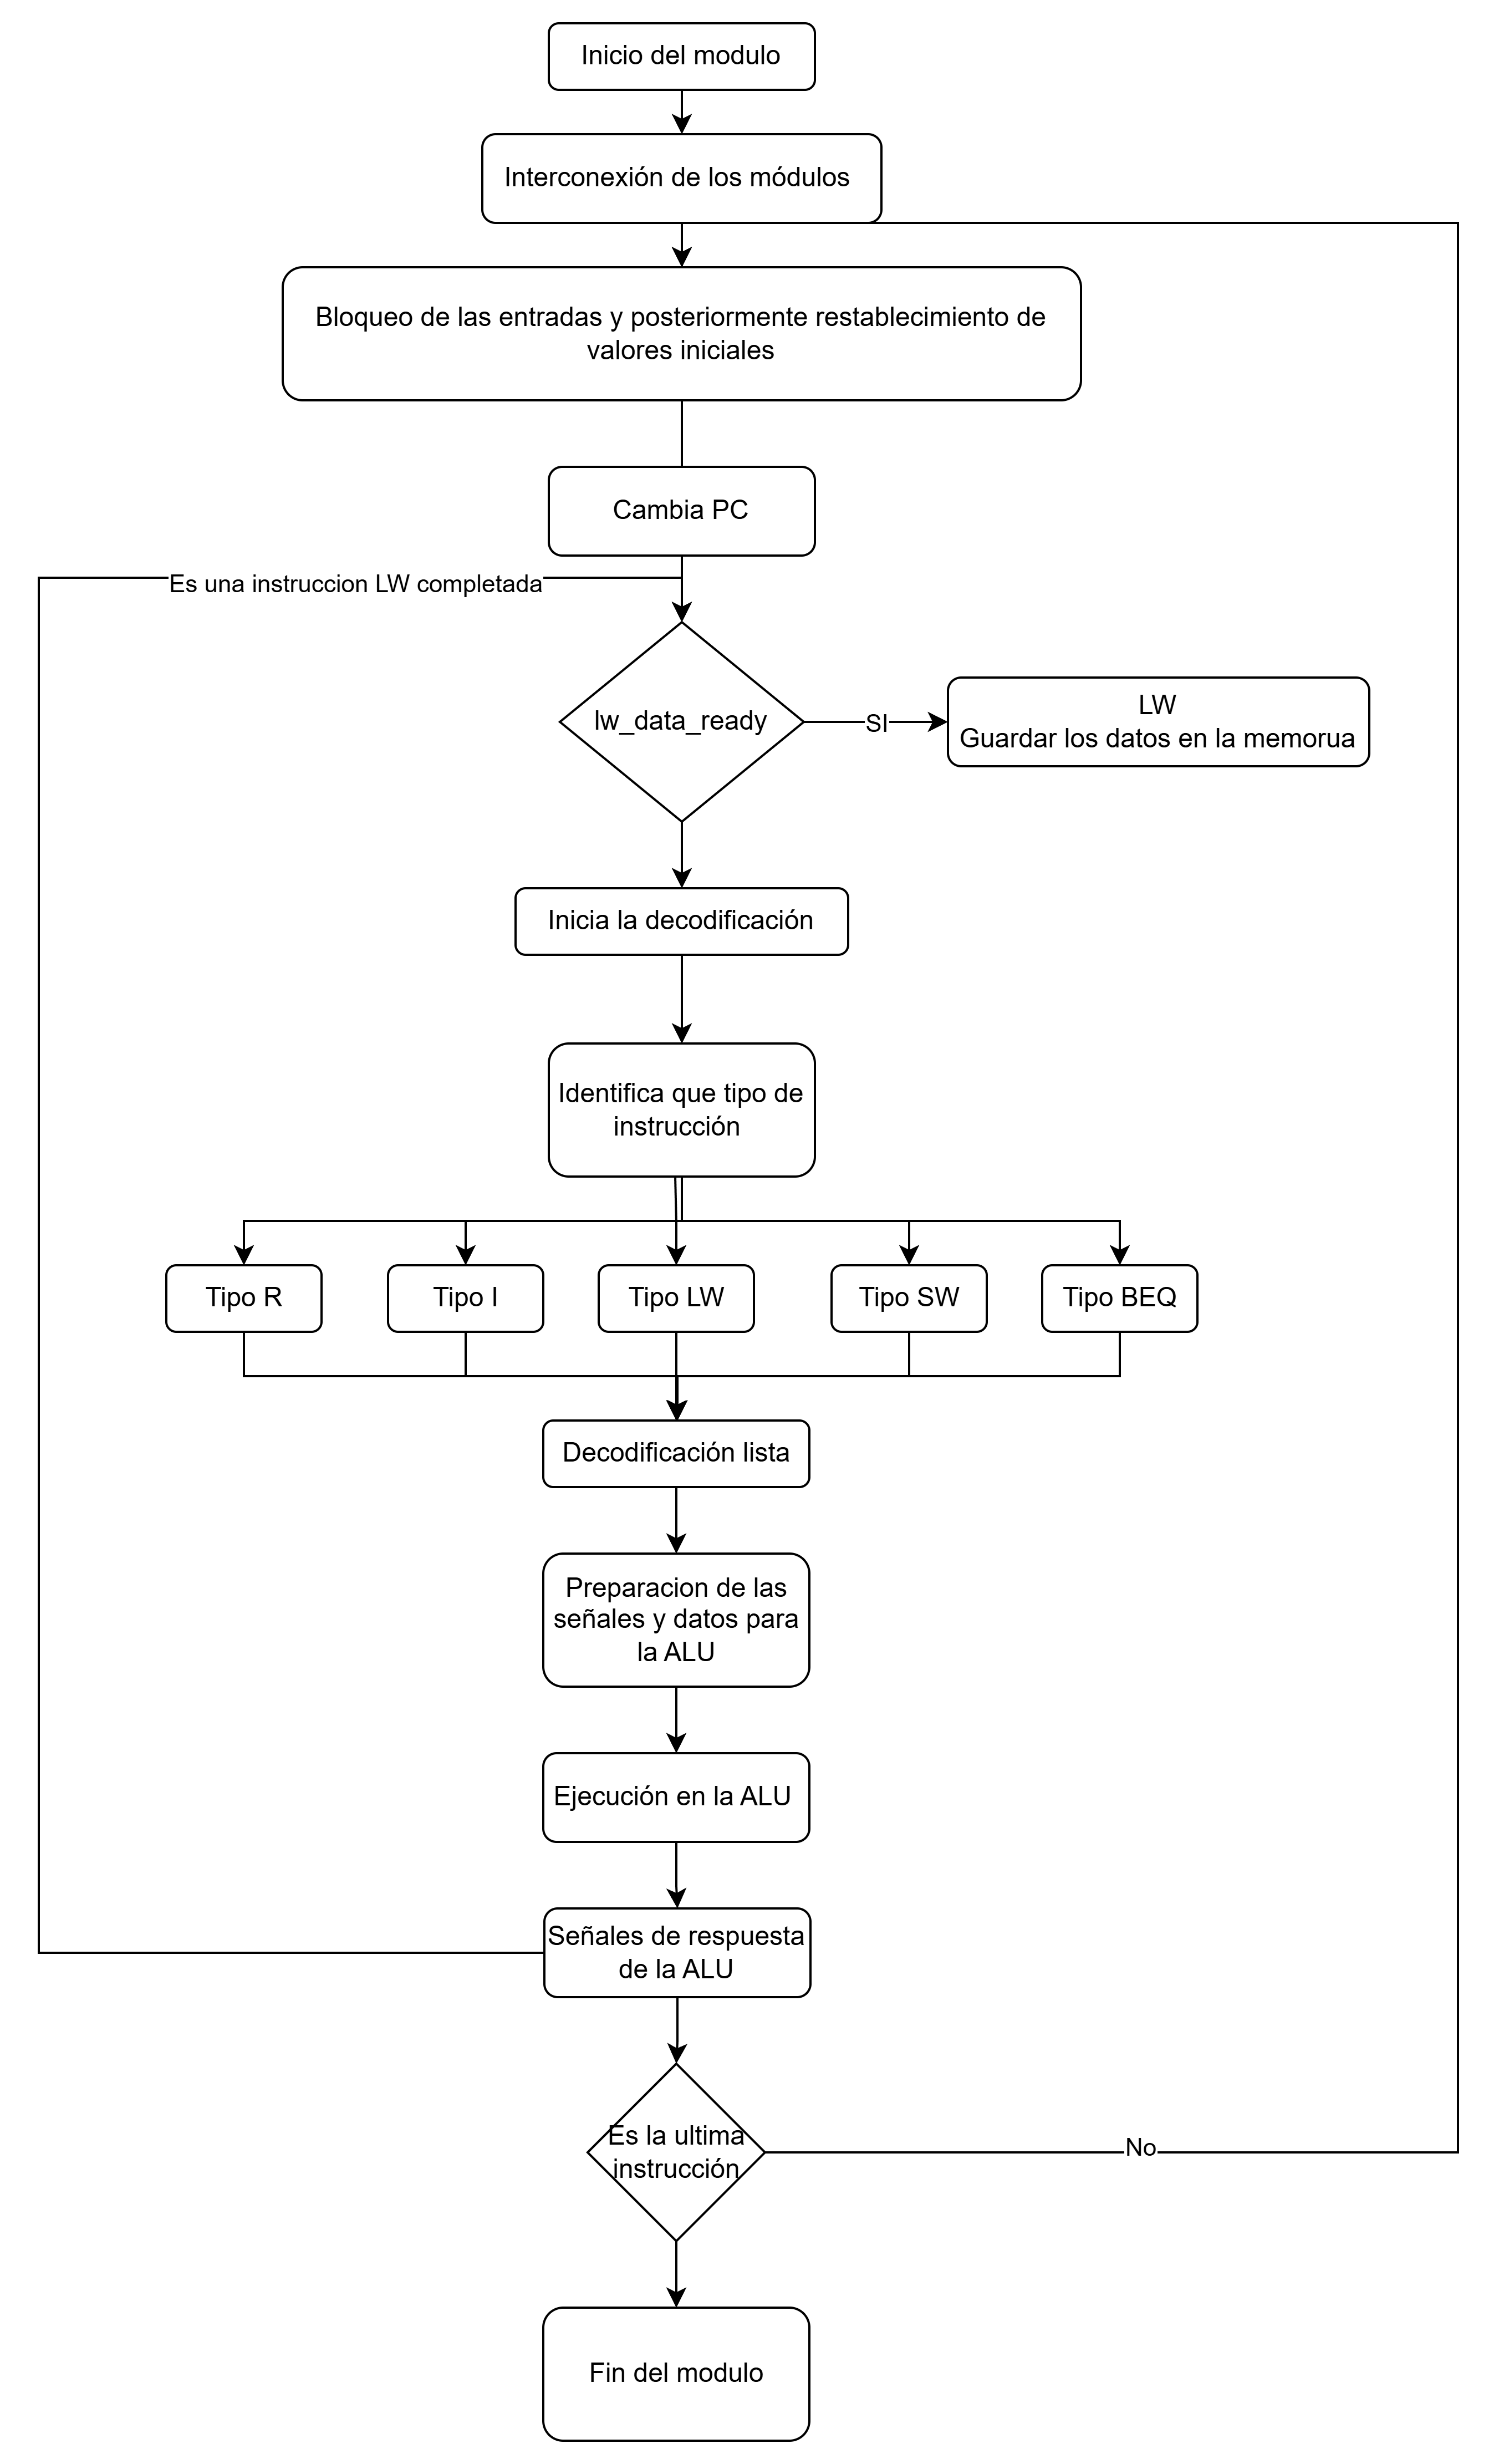
\includegraphics[width=0.95\linewidth]{Diagrama de flujo del modulo RISCVunicycle.png}
    \caption{Diagrama de flujo del módulo principal RISCVunicycle}
    \label{fig:diagrama-flujo-riscvunicycle}
\end{figure}

\subsubsection{Funcionamiento}
Obtiene instrucciones usando el PC y la Memoria de Instrucciones. La instruccion es decodificada por la unidad de control, que genera todas las senales de control para el datapath y la ALU. El datapath ejecuta la instruccion en un solo ciclo, utilizando la lógica de selección de operandos y actualizacion de PC adecuada según la instruccion (incluyendo saltos JAL y JALR). La arquitectura modular permite una mayor claridad y facilidad de depuración.

Una instruccion especial \texttt{32'hFFFFFFFF} actúa como senal de parada, activando \texttt{finish\_flag}.

\section{Cambios respecto a la versión anterior}
\label{sec:changes}
La versión anterior del procesador utilizaba una máquina de estados (FSM) embebida para la secuenciación de control. En la versión actual, la arquitectura ha sido completamente modularizada:
\begin{itemize}
    \item La lógica de control es ahora completamente combinacional y reside en un módulo independiente (\texttt{control\_unit.sv}).
    \item El camino de datos está abstraído en el módulo \texttt{datapath.sv}, que recibe todas las senales de control de manera explícita.
    \item Se ha añadido un módulo \texttt{alu\_control.sv} para la decodificación de operaciones de la ALU.
    \item El manejo de instrucciones de salto (JAL/JALR) se ha centralizado en la unidad de control, eliminando lógica redundante en el datapath.
    \item Todas las senales de control se asignan explícitamente para cada instruccion, evitando valores indeterminados.
    \item El diseño es ahora más claro, escalable y fácil de mantener.
\end{itemize}

\section{Conjunto de Instrucciones Implementado}
\label{sec:instruction_set}
El procesador soporta las siguientes instrucciones RISC-V:

\begin{itemize}
    \item \textbf{Transferencia de datos:}
    \begin{itemize}
        \item \texttt{lw}  (Load Word)
        \item \texttt{sw}  (Store Word)
    \end{itemize}
    \item \textbf{Desplazamientos:}
    \begin{itemize}
        \item \texttt{sll}, \texttt{slli}  (Shift Left Logical)
        \item \texttt{srl}, \texttt{srli}  (Shift Right Logical)
        \item \texttt{sra}, \texttt{srai}  (Shift Right Arithmetic)
    \end{itemize}
    \item \textbf{Aritméticas y lógicas:}
    \begin{itemize}
        \item \texttt{add}, \texttt{addi}, \texttt{sub}
        \item \texttt{xor}, \texttt{xori}
        \item \texttt{or}, \texttt{ori}
        \item \texttt{and}, \texttt{andi}
    \end{itemize}
    \item \textbf{Saltos condicionales:}
    \begin{itemize}
        \item \texttt{beq}, \texttt{bne}, \texttt{blt}, \texttt{bge}
    \end{itemize}
    \item \textbf{Comparaciones:}
    \begin{itemize}
        \item \texttt{slt}, \texttt{slti}
        \item \texttt{sltu}, \texttt{sltui}
    \end{itemize}
    \item \textbf{Saltos incondicionales:}
    \begin{itemize}
        \item \texttt{jal}, \texttt{jalr}
    \end{itemize}
\end{itemize}

% Aquí pueden añadirse ejemplos detallados para cada tipo de instruccion.

\section{Resultados}

Para la simulación del procesador, se utilizaron los archivos \texttt{Test1.hex} y \texttt{Test2.hex} como ejemplos de memoria de instrucciones, y el archivo \texttt{ProyectoCorto\_data.hex} como memoria de datos.

En el Apéndice se incluyen los ejemplos completos de los archivos de memoria de instrucciones Test1.hex y Test2.hex utilizados en la simulación.

\textbf{Contenido de ProyectoCorto\_data.hex (memoria de datos):}

\begin{lstlisting}[language=]
00000005
00000006
00000000
00000001
\end{lstlisting}

Estos archivos contienen, respectivamente, el conjunto de instrucciones a ejecutar y los datos necesarios para las operaciones de carga y almacenamiento durante la simulación.


Los resultados completos de la salida obtenida en la simulación del procesador pueden consultarse en el apéndice.

\section{Conclusión}
\label{sec:conclusion}
Este documento ha descrito el diseño e implementación de un procesador RISC-V uniciclo, explicando la funcionalidad de cada módulo y su rol dentro de la arquitectura general. Tras la simulación, los resultados obtenidos muestran el correcto funcionamiento del procesador, evidenciando la ejecucion secuencial de instrucciones tipo I, R, S, B y LW, así como la interacción entre los módulos principales. El procesador soporta un subconjunto fundamental de instrucciones RISC-V, validando los principios básicos de un diseño uniciclo y permitiendo observar el flujo de datos y control en cada ciclo de instruccion.

Los resultados de las simulaciones realizadas con los archivos Test1.hex y Test2.hex confirman que el procesador ejecuta correctamente instrucciones aritméticas, lógicas, de carga, almacenamiento y salto. En el caso de Test1.hex, se pudo observar la correcta inicialización de registros, la ejecucion de operaciones matemáticas y el uso de instrucciones de control de flujo, lo que permitió verificar la secuencia esperada de estados internos del procesador. Por su parte, la simulación con Test2.hex demostró la capacidad del procesador para manipular datos en memoria, realizar intercambios y comparar valores, validando así el funcionamiento de instrucciones más complejas y la interacción entre los diferentes módulos.

Estos resultados no solo avalan la correcta implementación del camino de datos y la lógica de control, sino que también evidencian la robustez del diseño frente a diferentes escenarios de prueba. Sin embargo, existen oportunidades de mejora, como la ampliación del conjunto de instrucciones soportadas, la optimización del rendimiento y la incorporación de mecanismos de manejo de excepciones. En conclusión, el procesador desarrollado constituye una base sólida para futuras extensiones y experimentos en el ámbito del diseño de arquitecturas RISC-V.

\onecolumn
\section*{Apéndice}
\addcontentsline{toc}{section}{Apéndice}

A continuación se muestra el contenido de Test1.hex (memoria de instrucciones)::

\begin{lstlisting}[language=,basicstyle=\ttfamily\footnotesize]
addi x1, x0, 7      # Inicializa x1 con 7
addi x2, x0, -10    # Inicializa x2 con -10
lw x4, 1(x0)        # Carga el primer dato (0x00000005) desde memoria a x4
lw x5, 3(x0)        # Carga el segundo dato (0x00000006) desde memoria a x5
addi x0, x0, 0      # NOP
add x6, x4, x5      # Suma x4 y x5, guarda el resultado en x6
sw x6, 1(x0)        # Almacena el valor de x6 en la direccion 4 de memoria
beq x6, x1, begin   # Si x6 == x1, salta al inicio
addi x8, x0, 10     # Si no salta, inicializa x8 con 10 (fin del programa)
\end{lstlisting}

A continuación se muestra el contenido de Test2.hex (memoria de instrucciones)::

\begin{lstlisting}[language=,basicstyle=\ttfamily\footnotesize]
# Inicializa x1 con 0 (direccion A)
addi x1, x0, 0
# Inicializa x2 con 5 (direccion B)
addi x2, x0, 5

# Llama a la funcion swapp en memoria (intercambia memoria[x1] y memoria[x2])
jal x3, swapp

# Continua aqui tras el swap
# Carga el valor de memoria[x1] en x4
lw x4, 0(x1)
# Carga el valor de memoria[x2] en x5
lw x5, 0(x2)

# Compara si x4 < x5 usando SLT
slt x6, x4, x5

# Si x6 == 0 (x4 >= x5), termina
beq x0, x0, fin

# Si x6 != 0, inicializa x7 con 99 (demuestra que el swap fue exitoso)
addi x7, x0, 99

# --- Funcion swapp ---
swapp:
    # Carga memoria[x1] en x8
    lw x8, 0(x1)
    # Carga memoria[x2] en x9
    lw x9, 0(x2)
    # Guarda x9 en memoria[x1]
    sw x9, 0(x1)
    # Guarda x8 en memoria[x2]
    sw x8, 0(x2)
    # Retorna a la instruccion siguiente al JAL
    jalr x0, 0(x3)
fin:
# NOP para terminar
addi x0, x0, 0
\end{lstlisting}

A continuación se muestra el resultado completo obtenido en PowerShell al simular el procesador con Test1.hex:

\lstset{basicstyle=\footnotesize\ttfamily,breaklines=true}
\begin{lstlisting}[language=]
Memory initialized:
WARNING: src/datamem.sv:13: $readmemh(hex/ProyectoCorto_data.hex): Not enough words in the file for the requested range [0:255].
VCD info: dumpfile RISCVunicycle_tb.vcd opened for output.
[0] INFO: Reset Asserted.
[0] [PC] Reset: PC = fffffffc
[5000] [PC] Reset: PC = fffffffc
[15000] [PC] Reset: PC = fffffffc
[20000] INFO: Reset De-asserted.
[ALU_Control] Opcode no reconocido: xxxxxxx
[ALU_Control] ALU_Op resultante: 0011
[Control] Opcode: xxxxxxx, Funct3: xxx, Funct7: xxxxxxx, ALU_Zero: 0
[Control] INSTRUCCION: opcode desconocido: xxxxxxx
[Control] reg_we=0
[Control] mem_rd=0
[Control] mem_we=0
[Control] alu_src_b=0
[Control] mem_to_reg=00
[Control] branch=0
[Control] pc_src=00
[Control] jal_active=0
[Control] jalr_active=0

[PC] PC actualizado:          0
[InstMemory] addr:          0, Instruccion: 00700093
Inm ext mod side: 00000007
[ALU_Control] ALU_Op resultante: 0010
[RegisterFile] Read1: x0 =          0, Read2: x7 =          0
[Control] Opcode: 0010011, Funct3: 000, Funct7: 0000000, ALU_Zero: 0
[Control] INSTRUCCION: ADDI
[Control] reg_we=1
[Control] mem_rd=0
[Control] mem_we=0
[Control] alu_src_b=1
[Control] mem_to_reg=00
[Control] branch=0
[Control] pc_src=00
[Control] jal_active=0
[Control] jalr_active=0
[RegisterFile] Escritura: x1 =           7
[ALU] ALUctl = 0010
[ALU] Funcion: ADD
[ALU] A =           0
[ALU] B =           7
[ALU] ALUout =           7
[ALU] zero = 0
ADDI
R1:  0
D1:          0
alu_op: 0010
imm:     7
ext_imm:           7
Ejecutando operacion en la ALU
Aluin1:          0
Aluin2:          7
A:          0
B:          7
ALUctl: 0010
Resultado de la ALU:           7
Resultado listo para escritura en registro:           7
continuing to next instruction.
WriteData:           7
Inm ext mod side: fffffff6
addr:          4, Instruccion: ff600113

PC:           4
Instrucion: ff600113
opcode: 0010011
tipo I
Registro destino:  2
funct3: 0000
ADDI
R1:  0
D1:          0
alu_op: 0010
imm:   -10
ext_imm:         -10
Ejecutando operacion en la ALU
Aluin1:          0
Aluin2: 4294967286
A:          0
B: 4294967286
ALUctl: 0010
Resultado de la ALU:         -10
Resultado listo para escritura en registro:         -10
continuing to next instruction.
WriteData:         -10
addr:          8, Instruccion: 00102203

PC:           8
Instrucion: 00102203
opcode: 0000011
Load word
Registro destino:  4
alu_op: 0010
imm:     1
ext_imm:           1
Ejecutando operacion en la ALU
Aluin1:          0
Aluin2:          1
A:          0
B:          1
ALUctl: 0010
Resultado de la ALU:           1
Leyendo de memoria en direccion:          1
continuing to next instruction.
Cargando datos desde memoria:           6
addr:         12, Instruccion: 00302283
WriteData:           6
PC:          12
Instrucion: 00302283
opcode: 0000011
Load word
Registro destino:  5
alu_op: 0010
imm:     3
ext_imm:           3
Ejecutando operacion en la ALU
Aluin1:          0
Aluin2:          3
A:          0
B:          3
ALUctl: 0010
Resultado de la ALU:           3
Leyendo de memoria en direccion:          3
continuing to next instruction.
Cargando datos desde memoria:           1
addr:         16, Instruccion: 00000013
Inm ext mod side: 00000000

PC:          16
Instrucion: 00000013
opcode: 0010011
tipo I
Registro destino:  0
funct3: 0000
ADDI
R1:  0
D1:          0
alu_op: 0010
imm:     0
ext_imm:           0
Ejecutando operacion en la ALU
Aluin1:          0
Aluin2:          0
A:          0
B:          0
ALUctl: 0010
Resultado de la ALU:           0
Resultado listo para escritura en registro:           0
continuing to next instruction.
WriteData:           0
addr:         20, Instruccion: 00520333

PC:          20
Instrucion: 00520333
opcode: 0110011
tipo R
funct3: 0000
Registro destino:  6
ADD
R1:  4
R2:  5
D1:          6
D2:          1
alu_op: 0010
Data1:          6
Data2:          1
Ejecutando operacion en la ALU
Aluin1:          6
Aluin2:          1
A:          6
B:          1
ALUctl: 0010
Resultado de la ALU:           7
Resultado listo para escritura en registro:           7
continuing to next instruction.
WriteData:           7
addr:         24, Instruccion: 006020a3

PC:          24
Instrucion: 006020a3
opcode: 0100011
store word
alu_op: 0010
Data1:          0
Data2:          1
imm:     1
ext_imm:           1
Ejecutando operacion en la ALU
Aluin1:          0
Aluin2:          1
A:          0
B:          1
ALUctl: 0010
Resultado de la ALU:           1
Escribiendo en memoria en direccion:          1
Datos a escribir en memoria:           1
continuing to next instruction.
Inm ext mod side: ffffffe4
addr:         28, Instruccion: fe1302e3

PC:          28
Instrucion: fe1302e3
opcode: 1100011
branch?
alu_op: 0110
Data1:          7
Data2:          7
imm:   -14
ext_imm:         -28
Ejecutando operacion en la ALU
Aluin1:          7
Aluin2:          7
A:          7
B:          7
ALUctl: 0110
Resultado de la ALU:           0
Resultado listo para escritura en registro:           0
Branch taken, jumping to address:           0
...
\end{lstlisting}

A continuación se muestra el resultado completo obtenido en PowerShell al simular el procesador con Test2.hex:

\lstset{basicstyle=\footnotesize\ttfamily,breaklines=true}
\begin{lstlisting}[language=]
WARNING: src/instmemory.sv:22: $readmemh(hex/Test2.hex): Not enough words in the file for the requested range [0:31].
Memory initialized:
WARNING: src/datamem.sv:13: $readmemh(hex/ProyectoCorto_data.hex): Not enough words in the file for the requested range [0:255].
VCD info: dumpfile RISCVunicycle_tb.vcd opened for output.
[0] INFO: Reset Asserted.
[0] [PC] Reset: PC = fffffffc
[5000] [PC] Reset: PC = fffffffc
[15000] [PC] Reset: PC = fffffffc
[20000] INFO: Reset De-asserted.
[ALU_Control] Opcode no reconocido: xxxxxxx
[ALU_Control] ALU_Op resultante: 0011
[Control] Opcode: xxxxxxx, Funct3: xxx, Funct7: xxxxxxx, ALU_Zero: 0
[Control] INSTRUCCION: opcode desconocido: xxxxxxx
[Control] Opcode no reconocido: xxxxxxx
[Control] reg_we=0
[Control] mem_rd=0
[Control] mem_we=0
[Control] alu_src_b=0
[Control] mem_to_reg=00
[Control] branch=0
[Control] pc_src=00
[Control] jal_active=0
[Control] jalr_active=0
 
[PC] PC actualizado:          0
[InstMemory] addr:          0, Instruccion: 00000093
Inm ext mod side: 00000000
[ALU_Control] ALU_Op resultante: 0010
[RegisterFile] Read1: x0 =          0, Read2: x0 =          0
[Control] Opcode: 0010011, Funct3: 000, Funct7: 0000000, ALU_Zero: 0
[Control] INSTRUCCION: ADDI
[Control] reg_we=1
[Control] mem_rd=0
[Control] mem_we=0
[Control] alu_src_b=1
[Control] mem_to_reg=00
[Control] branch=0
[Control] pc_src=00
[Control] jal_active=0
[Control] jalr_active=0
[RegisterFile] Escritura: x1 =           0
[ALU] ALUctl = 0010
[ALU] Funcion: ADD
[ALU] A =           0
[ALU] B =           0
[ALU] ALUout =           0
[ALU] zero = 0

[PC] PC actualizado:          4
R1:  0
D1:          0
alu_op: 0010
A:          0
B:          0
ALUctl: 0010
imm:     0
ext_imm:           0
Ejecutando operacion en la ALU
Aluin1:          0
Aluin2:          0
Resultado de la ALU:           0
Resultado listo para escritura en registro:           0
continuing to next instruction.
WriteData:           0
Inm ext mod side: 00000005
addr:          4, Instruccion: 00500113

PC:           4
Instrucion: 00500113
opcode: 0010011
tipo I
Registro destino:  2
funct3: 0000
R1:  0
D1:          0
alu_op: 0010
imm:     0
ext_imm:           5
Ejecutando operacion en la ALU
Aluin1:          0
Aluin2:          5
A:          0
B:          5
ALUctl: 0010
Resultado de la ALU:           5
Resultado listo para escritura en registro:           5
continuing to next instruction.
WriteData:           5
addr:          8, Instruccion: 018001ef
Inm ext mod side: 00000018

PC:           8
Instrucion: 018001ef
opcode: 1101111
JAL
R1:  0
D1:          0
funct3: 0000
alu_op: 0010
WriteData:          12
Ejecutando operacion en la ALU
Aluin1:          0
Aluin2:         24
A:          0
B:         24
ALUctl: 0010
Resultado de la ALU:          24
Guardando direccion de retorno:          12
Jump taken, jumping to address:          32
addr:         32, Instruccion: 0000a403

PC:          32
Instrucion: 0000a403
opcode: 0000011
Load word
Registro destino:  8
alu_op: 0010
imm:     0
ext_imm:           0
Ejecutando operacion en la ALU
Aluin1:          0
Aluin2:          0
A:          0
B:          0
ALUctl: 0010
Resultado de la ALU:           0
Leyendo de memoria en direccion:          0
continuing to next instruction.
Cargando datos desde memoria:           x
addr:         36, Instruccion: 00012483
WriteData:           x

PC:          36
Instrucion: 00012483
opcode: 0000011
Load word
Registro destino:  9
alu_op: 0010
Data1:          5
Data2:          0
imm:     0
ext_imm:           0
Ejecutando operacion en la ALU
Aluin1:          5
Aluin2:          0
A:          5
B:          0
ALUctl: 0010
Resultado de la ALU:           5
Leyendo de memoria en direccion:          5
continuing to next instruction.
Cargando datos desde memoria:           x
addr:         40, Instruccion: 0090a023

PC:          40
Instrucion: 0090a023
opcode: 0100011
store word
alu_op: 0010
Data1:          0
Data2:          0
imm:     0
ext_imm:           0
Ejecutando operacion en la ALU
Aluin1:          0
Aluin2:          0
A:          0
B:          0
ALUctl: 0010
Resultado de la ALU:           0
Escribiendo en memoria en direccion:          0
Datos a escribir en memoria:           0
continuing to next instruction.
addr:         44, Instruccion: 00812023

PC:          44
Instrucion: 00812023
opcode: 0100011
store word
alu_op: 0010
Data1:          5
Data2:          0
imm:     0
ext_imm:           0
Ejecutando operacion en la ALU
Aluin1:          5
Aluin2:          0
A:          5
B:          0
ALUctl: 0010
Resultado de la ALU:           5
Escribiendo en memoria en direccion:          5
Datos a escribir en memoria:           0
continuing to next instruction.
Inm ext mod side: 00000000
addr:         48, Instruccion: 00018067

PC:          48
Instrucion: 00018067
opcode: 1100111
JALR
R1:  3
D1:         12
alu_op: 0010
Data1:         12
Data2:          0
WriteData:          52
Data1:         12
Data2:         52
Ejecutando operacion en la ALU
Aluin1:         12
Aluin2:          0
A:         12
B:          0
ALUctl: 0010
Resultado de la ALU:          12
Guardando direccion de retorno:          52
Jump taken, jumping to address:          12
addr:         12, Instruccion: 0000a203

PC:          12
Instrucion: 0000a203
opcode: 0000011
Load word
Registro destino:  4
alu_op: 0010
Data1:          0
Data2:         52
imm:     0
ext_imm:           0
Ejecutando operacion en la ALU
Aluin1:          0
Aluin2:          0
A:          0
B:          0
ALUctl: 0010
Resultado de la ALU:           0
Leyendo de memoria en direccion:          0
continuing to next instruction.
Cargando datos desde memoria:           0
addr:         16, Instruccion: 00012283
WriteData:           0

PC:          16
Instrucion: 00012283
opcode: 0000011
Load word
Registro destino:  5
alu_op: 0010
Data1:          5
Data2:         52
imm:     0
ext_imm:           0
Ejecutando operacion en la ALU
Aluin1:          5
Aluin2:          0
A:          5
B:          0
ALUctl: 0010
Resultado de la ALU:           5
Leyendo de memoria en direccion:          5
continuing to next instruction.
Cargando datos desde memoria:           0
addr:         20, Instruccion: 00522333

PC:          20
Instrucion: 00522333
opcode: 0110011
tipo R
funct3: 0010
Registro destino:  6
R1:  4
R2:  5
D1:          0
D2:          2
alu_op: 0111
Data1:          0
Data2:          2
A:          5
B:          0
ALUctl: 0111
Ejecutando operacion en la ALU
Aluin1:          0
Aluin2:          2
A:          0
B:          2
ALUctl: 0111
Resultado de la ALU:           1
Resultado listo para escritura en registro:           1
continuing to next instruction.
WriteData:           1
Inm ext mod side: 0000001c
addr:         24, Instruccion: 00000e63

PC:          24
Instrucion: 00000e63
opcode: 1100011
branch?
R2:  0
D2:         52
alu_op: 0110
Data1:         52
Data2:         52
A:          0
B:          2
ALUctl: 0110
imm:     0
ext_imm:          28
Ejecutando operacion en la ALU
Aluin1:         52
Aluin2:         52
A:         52
B:         52
ALUctl: 0110
Resultado de la ALU:           0
Resultado listo para escritura en registro:           0
Branch taken, jumping to address:          52
addr:         52, Instruccion: 00000013
Inm ext mod side: 00000000

PC:          52
Instrucion: 00000013
opcode: 0010011
tipo I
Registro destino:  0
funct3: 0000
R1:  0
D1:         52
alu_op: 0010
A:         52
B:         52
ALUctl: 0010
imm:     0
Ejecutando operacion en la ALU
Aluin1:         52
Ejecutando operacion en la ALU
Aluin1:         52
Ejecutando operacion en la ALU
Ejecutando operacion en la ALU
Aluin1:         52
Aluin2:          0
A:         52
B:          0
ALUctl: 0010
Resultado de la ALU:          52
Resultado listo para escritura en registro:          52
continuing to next instruction.
WriteData:          52
addr:         56, Instruccion: ffffffff

PC:          56
Instrucion: ffffffff
opcode: 1111111
alu_op: 0010
Esta es la ultima instruccion, terminando la simulacion.
./../src/RISCVunicycle.sv:382: $finish called at 1105000 (1ns)
Data1:          0
Test bench finished successfully.
\end{lstlisting}


\bibliographystyle{IEEEtran}
\bibliography{references} % This will point to a references.bib file

\end{document}
